%!TEX root = vaisagh_thesis.tex

\chapter{Validity check for Markov analysis}
\label{sec:validity_check_for_markov_analysis}

Chapter~\ref{chapter:SpatialKnowledgeChapter} introduced a novel Markovian analysis to analyse the use of memory in exploration. The effectiveness and validity of the Markovian analysis is, however, dependent on the amount of data available. The following experiments demonstrate the validity of the results obtained from the analysis.


\section{Effect of Dataset Size} % (fold)
\label{sec:effect_of_dataset_size}


In order to check whether the peak in the hop and coverage data is a function of the dataset size, we hypothesized that if the peak does not change on doubling the dataset size then the pattern that is seen is not an artifact of the dataset size. We plotted the same graph for $N=22$ (i.e. taking only 22 participants at random) and $N=44$ and checked if there is a shift in the peak to a higher value. As shown in Figure~\ref{fig:hop_and_coverage_for_different_n} there is clearly no shift. The peak value still remains at 7-8 and starts dropping at 9.

\begin{figure*}[!tb]
  \centering
   \subfloat[Hop and coverage for 44 players]{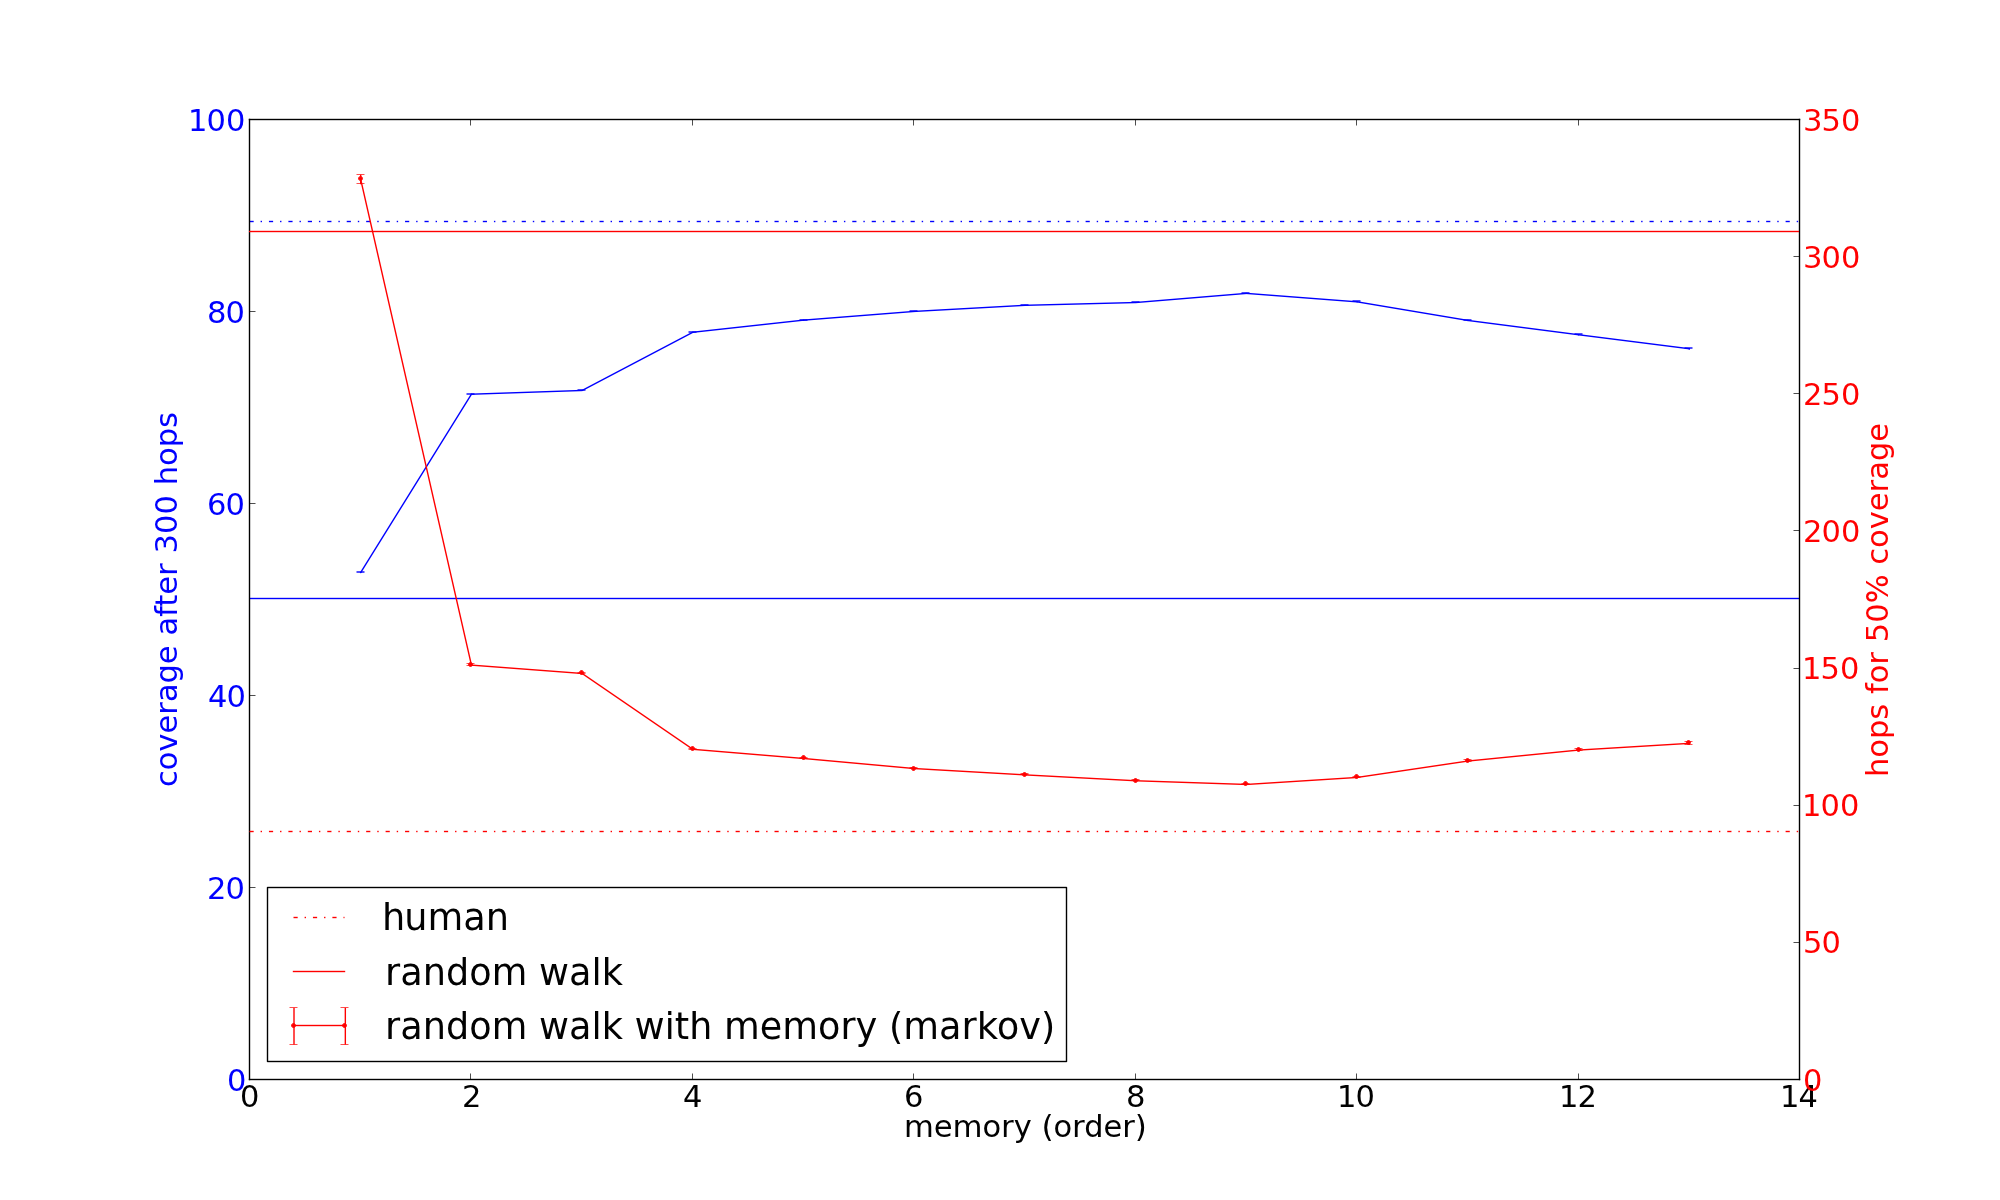
\includegraphics[width=5in]{SpatialKnowledge/44.PNG}}

  \subfloat[Hop and coverage for 22 players]{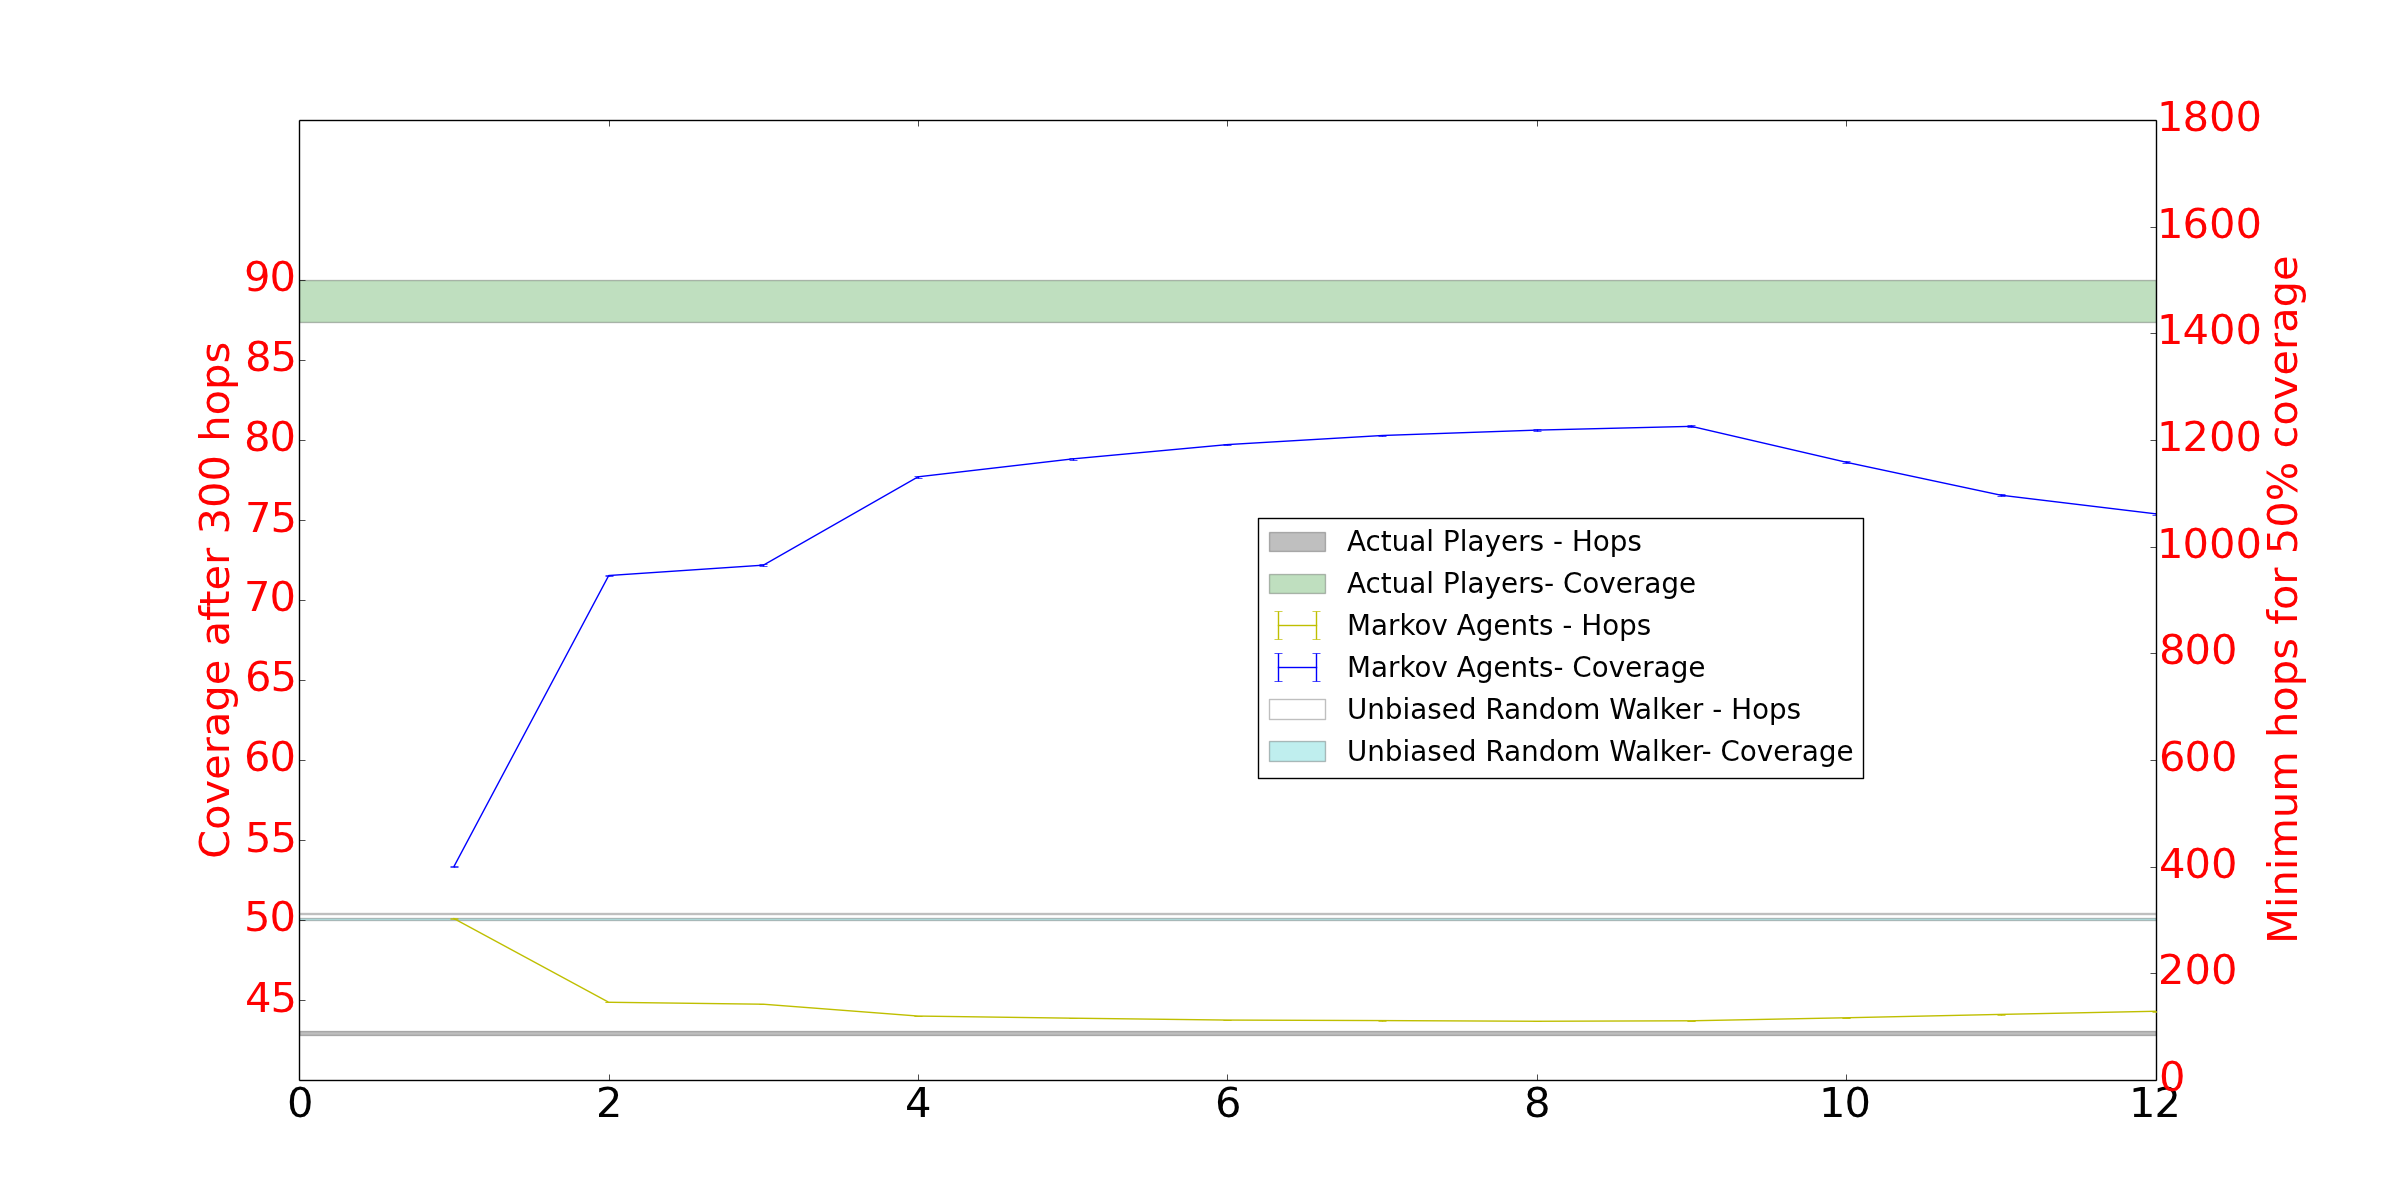
\includegraphics[width=5in]{SpatialKnowledge/22.PNG}}
  \caption[Dataset size dependence of calculations]{Hop and coverage graphs for different size of datasets seems to indicate that the peak is not dependent on data size.}
  \label{fig:hop_and_coverage_for_different_n}
\end{figure*}

\section{Decision Base Size at Decision Points} % (fold)
\label{sec:decision_base_size_at_decision_points}

\begin{figure*}[!tb]
    \begin{center}
        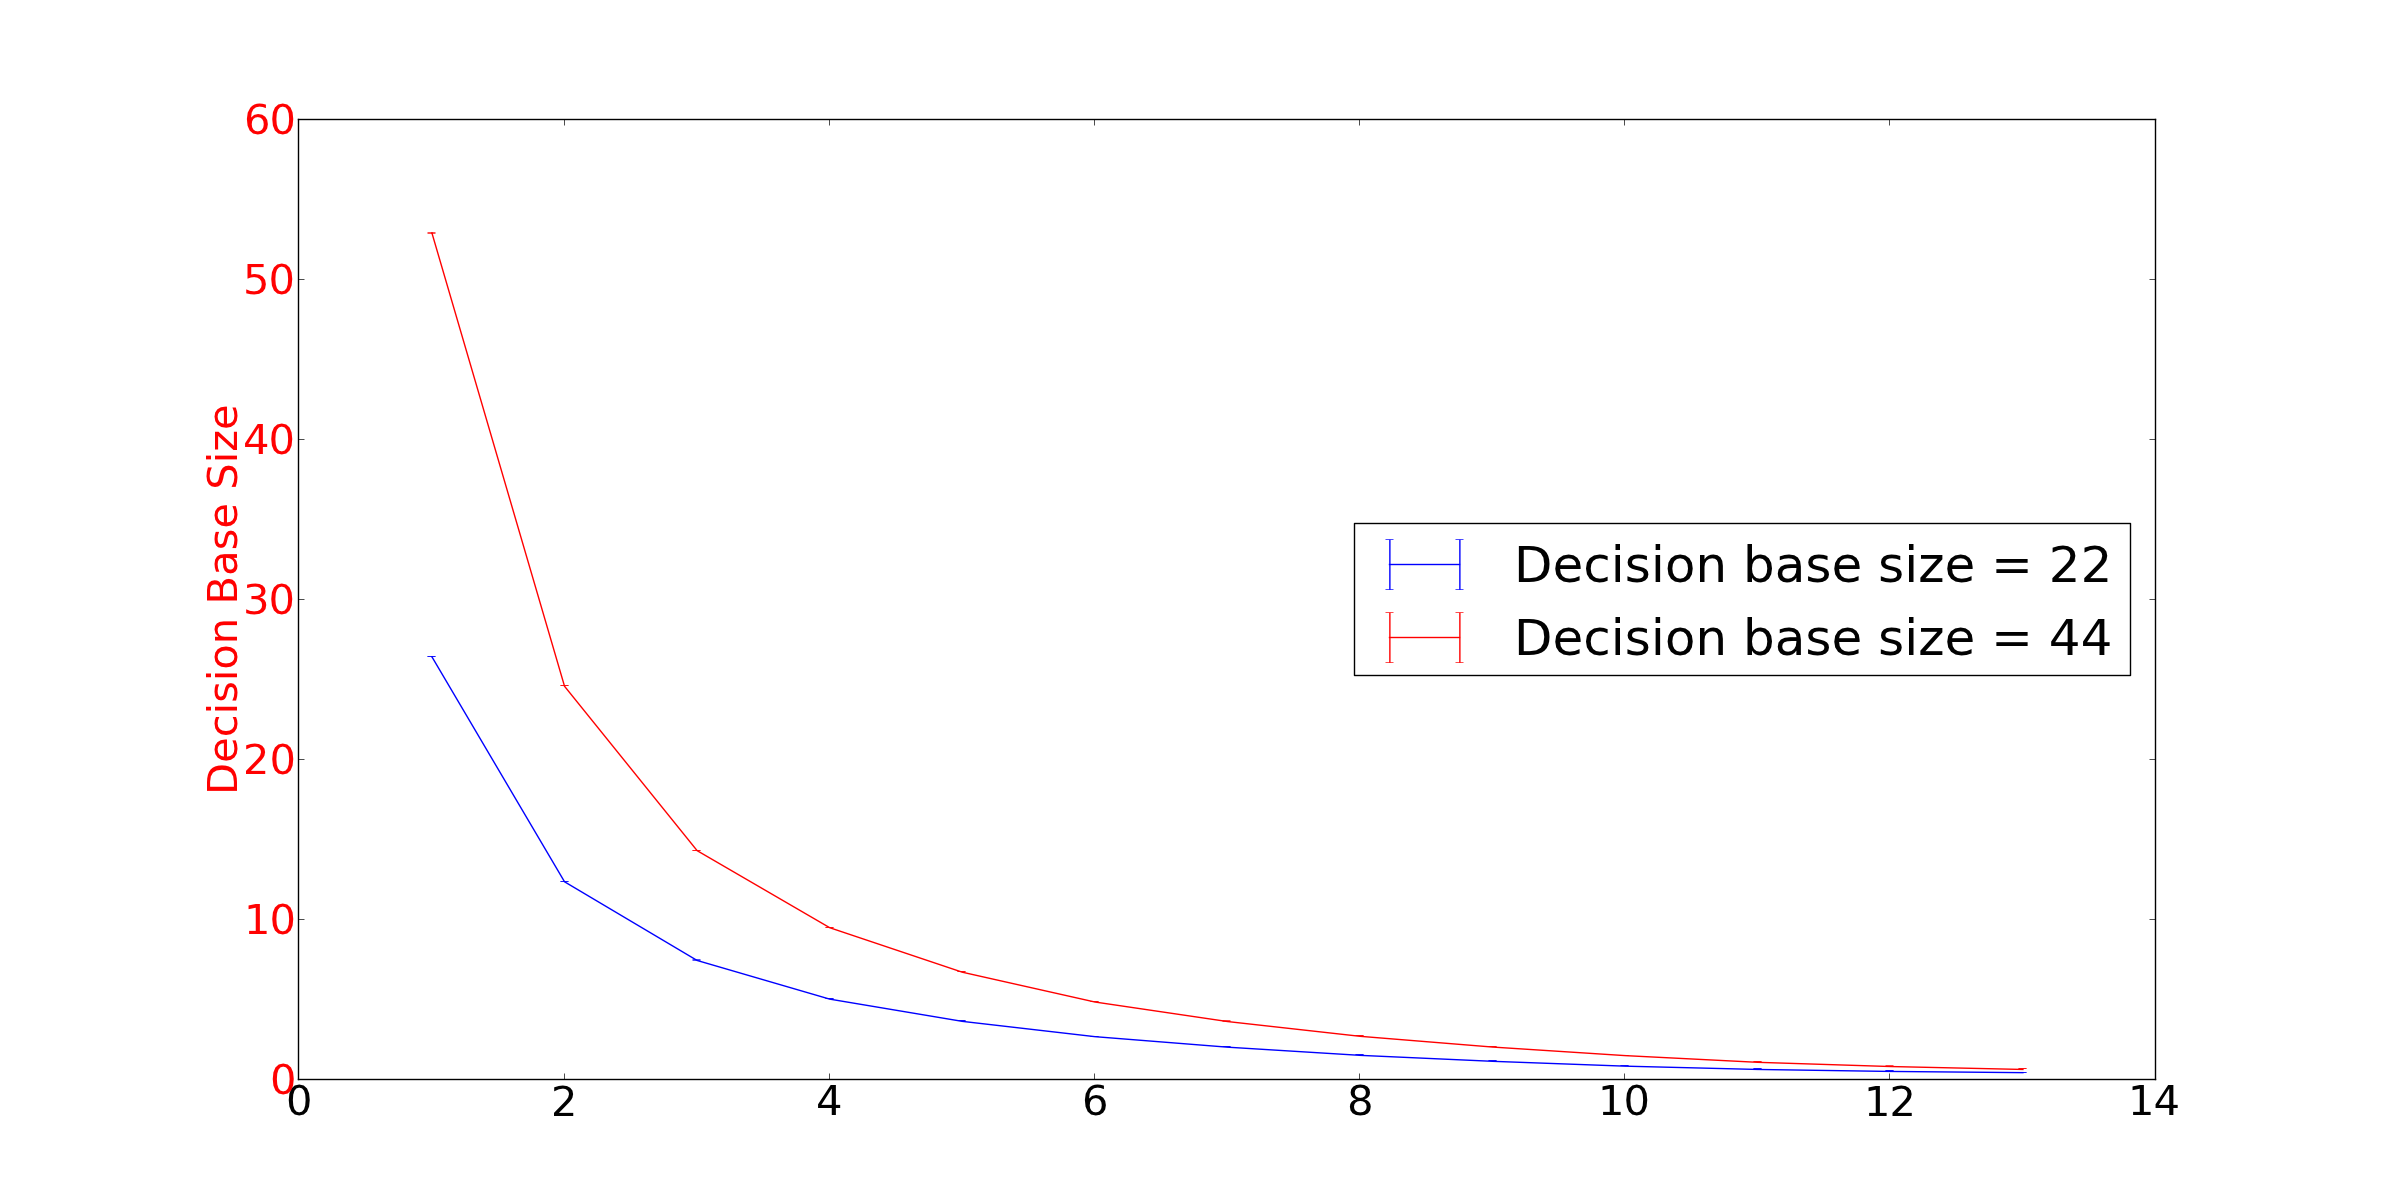
\includegraphics[width=5in]{SpatialKnowledge/decision-base.png}
    \end{center}
    \caption{Comparison of the decision base sizes.}
    \label{fig:decision_base_comparison}
\end{figure*}

The Markov data calculation (explained in Section~\ref{sec:Markov_data_analysis}) is based on aggregating the actions of the players at each decision point. The quality of the Markov data probability distribution calculated is thus based on the amount of data available to make predictions. In order to calculate an $m^{th}$ order probability of the next step, the calculations are done using the number of times the preceding sequence of $m$ steps occurred and the choices made at that point by players in the dataset. Thus, as the frequency of said path decreases, there is lesser data for the probability calculation. The $m^{th}$ order Markov calculation becomes progressively less reliable and less different from random noise as $m$ increases due to the limited size of the dataset.

To estimate the maximum value of $m$ for which $m^{th}$ order calculations can be done reliably we calculate the \emph{decision base size} of the calculations.

To calculate the decision base size for order $m$, we do the following: First, $30,000$ paths of $300$ hops are generated for an $m^{th}$ order Markov agent based on the dataset of size $N$. For each node in each path generated, the number of players that have actually made a decision at that point is counted. We divide this value by the number of decisions that are possible at that point. So a single decimal value is obtained for each node of each path generated. The average of this over all nodes a path gives the \emph{path specific decision base}.  The average of these path specific decision bases gives the decision base for the order $m$ and dataset of size $N$. The result of this calculation is shown in Figure~\ref{fig:decision_base_comparison}.

The figure, firstly and most importantly, shows the usefulness of having a larger dataset in the Markov data calculation. Also, beyond the $9^{th}$ order a decision base of size less than 2 is available indicating there are less than twice as many actions as there are choices on average at each decision point. This indicates that beyond the $9^{th}$ order the calculations are unreliable.



